\subsubsection{Lobby Menu}
Sơ đồ use-case Lobby Menu:
\begin{figure}[H]
    \centering
    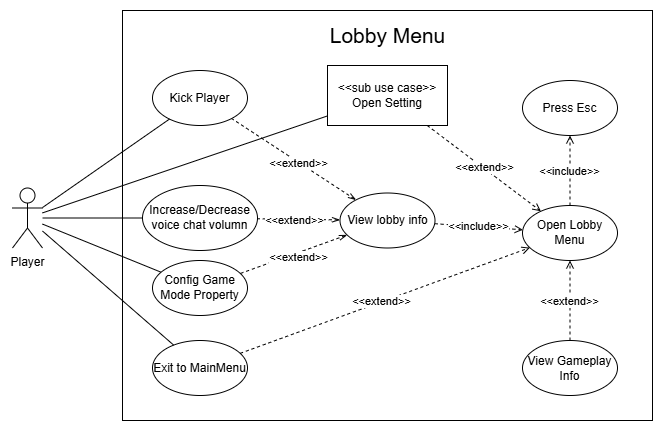
\includegraphics[width=0.75\linewidth]{4.Đặc tả chi tiết các lược đồ/Use-case/images/LobbyMenu.png}
    \caption{Use-case mô tả Lobby Menu}
    \label{fig:placeholder}
\end{figure}


\begin{table}[H]
\centering
\begin{tabular}{|p{4cm}|p{10cm}|}
\hline
\textbf{Use-case name} & Lobby Menu \\ \hline
\textbf{Actor} & Người chơi \\ \hline
\textbf{Descriptions} & Use-case này sẽ chỉ ra các luồng thực thi sau khi mở Lobby Menu. \\ \hline
\textbf{Pre-conditions} & Phải vào được trong lobby \\ \hline
\textbf{Trigger} & Người chơi nhấn nút “Esc” sau khi đã vào lobby. \\ \hline
\textbf{Post-conditions} & Người chơi chọn hành động mà mình muốn thực hiện \\ \hline
\textbf{Normal Flow} &
\begin{enumerate}
\item Người chơi nhấn nút \textbf{"Esc"} mở Lobby Menu.
\item Người chơi chọn các hành động player muốn.
\item Người chơi nhấn nút \textbf{"Esc"} để đóng Lobby Menu
\item Use-case kết thúc sau khi Lobby Menu được đóng thành công.
\end{enumerate}
\\ \hline
\textbf{Alternative Flow} &
\begin{enumerate}
\item[A1.] Sau khi mở được Lobby Menu, nếu người chơi muốn kick player khác thì người chơi nhấn "LOBBY INFO" sau đó chọn người chơi muốn kick và nhấn dấu x (chỉ chủ phòng mới có thể kick).
\item[A2.] Sau khi mở được Lobby Menu, nếu người chơi muốn Tăng/giảm âm lượng voice thì người chơi nhấn "LOBBY INFO", sau đó người tăng/giảm âm lượng voice chat của người chơi khác hoặc chính mình.
\item[A3.] Sau khi mở được Lobby Menu, nếu người chơi muốn điều chỉnh thông số của game mode thì người chơi nhấn "LOBBY INFO", sau đó nhấn nút nút mũi tên ">" rồi chọn game mode và điều chỉnh thông số của mode đó.
\item[A4.] Sau khi mở được Lobby Menu, nếu người chơi muốn thoát ra màn hình chính (rời khỏi phòng) thì người chơi nhấn nút "LEAVE GAME".
\item[A5. ] Sau khi mở được Lobby Menu, nếu người chơi muốn mở setting thì người chơi nhấn nút "SETTINGS".
\end{enumerate}
\\ \hline
\textbf{Exception Flow} &
Không có
\\ \hline
\end{tabular}
\end{table}